\chapter{Estrategias}

Para resolver un buen problema de olimpiada, debes esforzarte 
en encontrar la combinación correcta de tácticas matemáticas 
con las estrategias adecuadas. La estrategia suele no ser matemática, 
pueden aplicarse a problemas de todo tipo.

Especialmente si eres principiante, la estrategia posee gran importancia. 
Ante un problema difícil, regularmente no se sabe por donde empezar. 
Las estrategias psicológicas ayudan a despejar la mente y otras 
estrategias facilitan la investigación del problema. 
Una vez empezamos a trabajar, 
un marco estratégico ayuda a completar la solución.

Empezarémos con las estrategias psicológicas que se pueden aplicar a 
casi todos los problemas. Esto no significa que sean sencillas de dominar 
pero una vez las empezamos a contemplar, notaremos un rápido incremento 
de nuestra habilidad para trabajar en problemas. Hay que notar que no 
se promete un incremeneto en la habilidad para \textit{resolver problemas}, 
eso vendrá con el tiempo; pero, primero hay que trabajar duro :)

\section{Estrategias Psicológicas}

\subsection{El Ratón de Pólya}

Resumiré las ideas con el pequeño cuento, "Hombres y ratones" de 
George Pólya, el gran matemático y maestro de la resolución de problemas
(p. 75).

\begin{adjustwidth}{2cm}{}
    La casera se apresuró a entrar en el patio trasero, 
    puso la ratonera en el suelo (era una trampa antigua, 
    una jaula con trampilla) y llamó a su hija para que trajera al gato. 
    El ratón en la trampa, pareció comprender lo esencial de 
    estos procedimientos. Corrió frenéticamente en su jaula,
    se lanzó violentamente contra los barrotes; de un lado al otro; 
    y en el último momento, consiguió estrecharse a través de la jaula
    y desaparecerse en el campo del vecino. En ese lado de la ratonera, 
    debía de haber entre los barrotes una abertura un poco más ancha.
    En silencio felicité al ratón. Había resuelto un gran
    problema, y dio un gran ejemplo.

    De ese modo resolvemos problemas. Debemos intentar e intentar hasta que 
    eventualmente reconozcamos la diferencia entre varias aperturas 
    de lo que todo depende. Debemos variar nuestros caminos hasta que 
    exploremos todos los lados del problema. 

    El método fundamental entre hombres y ratones es el mismo: intentar, 
    e intentar de nuevo todos los caminos sin perdernos las pocas posibilidades 
    favorables. Es cierto los hombres son mejores resolviendo problemas que 
    los ratones. Un hombre no se lanza todo su cuerpo contra el obstáculo, 
    lo resuelve mentalmente; varía sus caminos aprendiendo más de sus 
    caminos fracasados que un ratón.
\end{adjustwidth}

La moraleja obviamente es: 

\begin{moral}
    Un tronador de problemas no se rinde fácilmente. 
\end{moral}

Sin embargo, no está tontamente golpeando su cabeza contra una pared 
(o caja), sino, hace varios intentos. Es claro que esto está muy 
simplificado.  Hay problemas que simplemente no puedes resolver. 
Tendrás que darte por vencido, al menos tempalmente y seguir con la vida. 
A veces hay que aceptar la derrota.

PERO, ¡la mayoría de principiantes se rinden muy pronto! 
Esto puede deberse por la falta de \textbf{confianza} y \textbf{concentración}. 
Es difícil trabajar en un problema si crees que no puedes resolverlo, y 
es imposible hacerlo si entraste en el \textit{umbral de frustración}. 
Es importante trabajar la \textbf{fortaleza mental} junto a las habilidades 
matemáticas para que el progreso sea significativo.

No es difícil adquirir una cantidad modesta de fortaleza mental. 
Puede que creas que contruir confianza es complicado y delicado, 
pero no estamos hablando de autoestima o sexualidad o cualquier cosa de 
ese tipo. Este no es un libro de autoayuda. Los problemas de matemáticas 
son bastanteeee más sencillos de lidiar con. Ya debes ser al menos un poco 
confiado sobre tu habilidad matemática, de otra forma no estarías aquí, 
leyendo el libro. Aun así, la fortaleces trabajando primero en problemas 
que te cuestan pero puedes resolver con una cantidad humilde de esfuerzo. 
Mientras trabajes en problemas en lugar de ejercicios, tu cerebro se 
ejercita, y tu subconsciente se acostumbra al éxito. 
Tu confianza crece automáticamente.

Con forme tu confianza crezca, también tu umbral de frustración lo hará 
si sigues incrementando tu \textit{carga} intelectual. Es algo que 
debemos aprender a frontar.
Empieza con problemas sencillos para calentar, pero debes trabajar 
en problemas más complicados y más monstrusos y más y más y más 
continuamente retando y estirando tu límite. Si un problema es interesante, 
no te importará estirar tu límite en ellos. Al inicio, te cansarás 
inmediatamente, con solo unos minutos de haber pensado en él. Pero 
llegará un punto donde estarás aferrado a un solo problema días, e 
incluso SEMANAS. 

\begin{figure}[h]
    \centering
    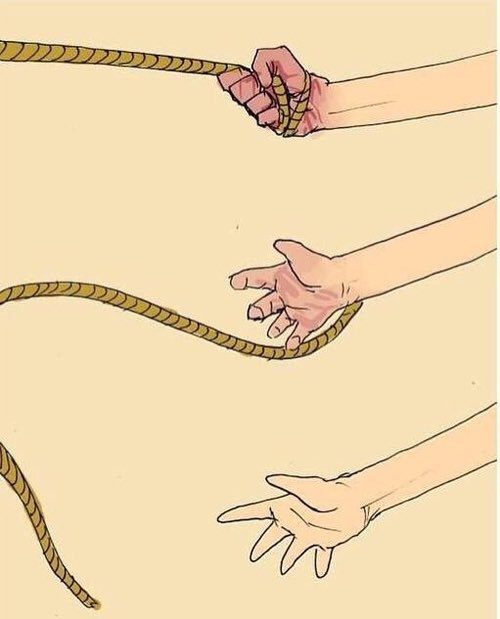
\includegraphics[height=6cm]{givingup.jpg}
    \caption{A veces aferrarse hace más daño que soltar}
\end{figure}

Hay problemas que te dejan traumado pero, ¿qué es más divertido que 
pensar en problemas retadores lo más seguido posible? ¿verdad? \dots
¿VERDAD? Además, ese trauma quedará muy grabado en tu memoria y 
siempre recordarás como se resolvía ese problema. Solo cuando un problema 
nos cuesta, valoramos su solución, y por lo tanto, aprendemos más de él.

\subsection{Creatividad}

Primero, revisemos un poco de filosofía muchachos. Platón creía que 
el conocimiento es innato, es decir que ya existe en nosotros y 
nuestro trabajo es "descubrirlo" en lugar de "crearlo". Nos es conveniente 
adoptar esa percepción. Al resolver un problema, tratar de encontrar 
la solución que ya está allí. Por esto, hay que ser altamente abieto 
y receptivo a nuevas ideas que flotan por ahí en nuestra visión. 
Que son invisibles para la mayoría de personas. 

A esta recepción de ideas escurridizas se le llama \textit{creatividad}. 
Observarla en acción es como un show de magia , donde cosas maravillosas 
suceden de un modo difícil de explicar . Veamos un ejemplo de un 
problema muy bonito cuya solución es inesperada.

\begin{example}
    Un monje escala una montaña. Empieza a las 8 am y alcanza la cima 
    al mediodía. La siguiente mañana, deja la cima a las 8 am y baja 
    por exactamente la misma ruta que tomó el día anterior, alcanzando 
    la base al mediodía. ¿Existe un momento entre las 8 am y el mediodía 
    en el que el monje estuvo en exactamente en el mismo lugar ambos días?
    (Nótese que no se menciona nada respecto a la velocidad a la que va 
    el monje, puede ir a 1000km por hora en los primeros minutos, después
    sentarse por una hora, después bajar un poco, etc. Tampoco menciona 
    que lleve la misma velocidad ambos días)
\end{example}

Sí, existe un momento en el que el monje estuvo en el mismo lugar 
ambos días.

\begin{proof}
    Deja al monje escalar la montaña del modo que deseé. Al insante en que 
    empiece a decender la montaña el segundo día, haz que otro monje 
    empiece a subirla desde la base en exactamente el modo en que el 
    primer monje la subió el día anterior. En algun punto, ambos monjes 
    se cruzaran. Ese es el momento y lugar que queríamos. 
\end{proof}

Lo extraordinario del problema es la fumada del segundo monje. La idea 
parece salir de la nada y aun así, resuelve el problema.

Esa es la creatividad en acción. La reacción natural ante ver esa solución
imaginativa es: "Wow, ¿cómo se le ocurrió? Yo jamás lo hubiera hecho." 
Mientras que es cierto, que hay gente más creativa que otra, siguiendo a 
Platón, ¡todos podemos aprender a ser creativos! Parte de este proceso 
viene de cultivar confianza, que ya revisamos su importancia.

\begin{moral}
    Aprende a apropiarte descaradamente de nuevas ideas y ha hacerlas 
    tuyas.
\end{moral}

No hay nada de malo con ello. Si son ideas hermosas, deberías 
dominarlas con entusiasmo y usarlas lo más seguido que puedas, tratando 
de ampliarlas y usarlas de modos novedosos. Siempre busca nuevas ideas. 
Cada problema debería verse como material de \textbf{idea novedosa}. 
Entre más te acostumbres a apropiarte y manipular ideas, es más 
probable que puedas crear las propias. 

Una forma de elevar tu receptividad de nuevas ideas es mantenerte 
"suelto", cultivar una especie de visión periférica. Debes relajar 
tu visión y obtener ideas que no estén a la vista directamente. Como 
el ratón de Pólya, constantemente buscar nuevos giros y trucos. 
No te cierres a un método.

\begin{moral}
    Rompe o dobla las reglas.
\end{moral}

\section{Estrategias Generales}

Vamos a revisar tres estrategias fundamentales que se pueden aplicar 
a problemas de cualquier tipo. Cada una será ejemplificada con 
un problema para \textit{facilitar} su comprensión

\subsection{¡Hazlo Más Fácil!}

\begin{example}
    En el siguiente diagrama, ¿Puedes conectar par de cajitas con la misma 
    letra con una línea sin que se cruze con otra línea?
\end{example}

\begin{figure}[h]
    \centering
    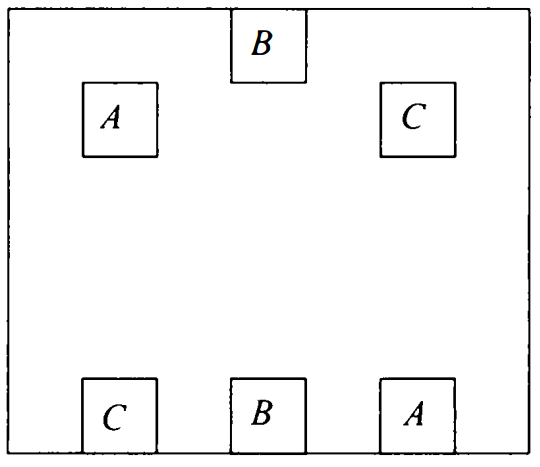
\includegraphics[height=3cm]{makeiteasierexample.png}
\end{figure}

La dificultad del problema parece radicar en que las cajas de arriba 
con la A y la C parecen estar volteadas, ¿no? Así que, ¿por qué no 
voltearlas y convertir el problema en uno trivial?

\begin{figure}[h]
    \centering
    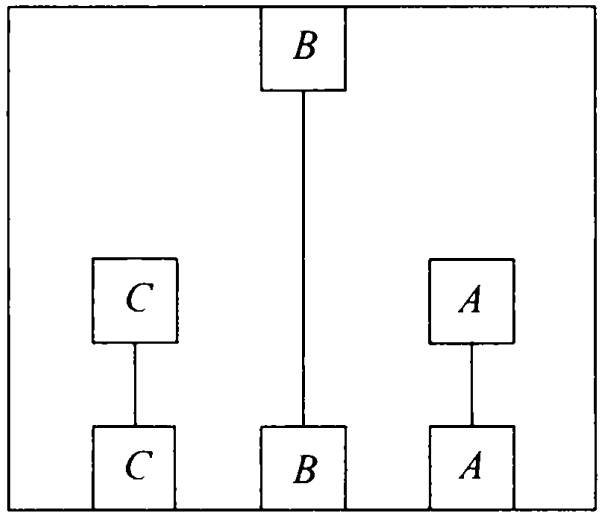
\includegraphics[height=3cm]{makeiteasier1.png}
\end{figure}

\begin{moral}
    Si un problema es muy complicado, simplifícalo.
\end{moral}

Por supuesto que no hemos resuelto el problema original. ¿O sí? 
Podemos "empujar" las cajas flotantes una a la vez. Primelo la A,

\begin{figure}[h]
    \centering
    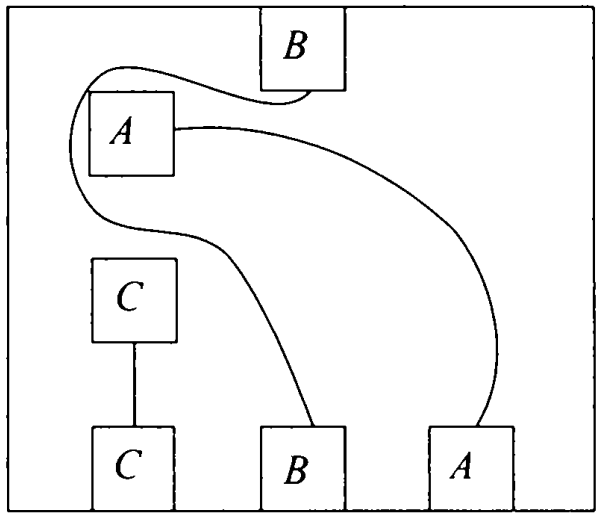
\includegraphics[height=3cm]{makeiteasier2.png}
\end{figure}

ahora, la C,

\begin{figure}[!h]
    \centering
    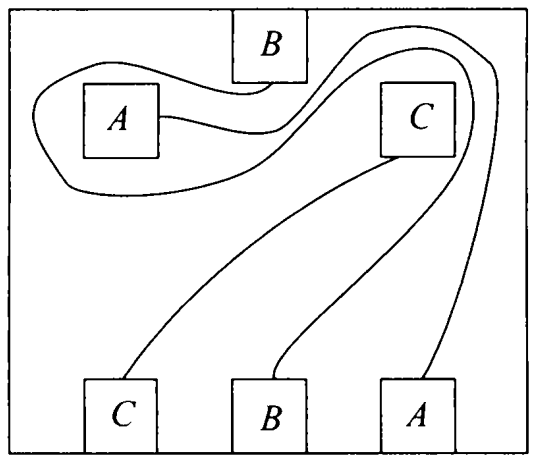
\includegraphics[height=3cm]{makeiteasier3.png}
\end{figure}

y hemos resuelto el problema.

\subsection{¡Liberate de los Límites Artificiales!}

\begin{example}
    Conecta los nueve puntos de el diagrama de abajo con un camino 
    ininterrumpido de 4 líneas rectas.
\end{example}

\begin{figure}[!h]
    \centering
    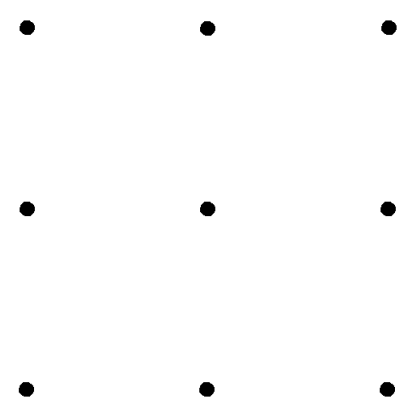
\includegraphics[height=3cm]{ninepoints.png}
\end{figure}

Cómo dice el título, !libérate de el límite artificial!, 
en este caso, de que solo hay nueve puntos. Una vez decides 
hacer líneas más allá de este límite, el problema es 
bastante fácil.

\begin{figure}[!h]
    \centering
    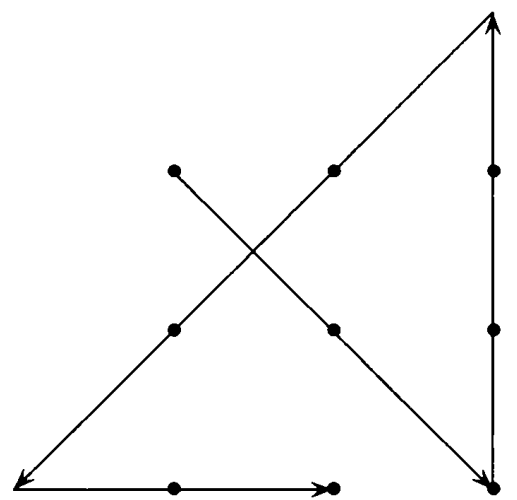
\includegraphics[height=3cm]{ninepointssolved.png}
\end{figure}

\subsection{¡Busca Patrones!}

\begin{example}
    Rellena la siguiente columna de la tabla.

    \vspace{2mm}
    \begin{center}
        \begin{tabular}{ |c|c|c|c|c|c|c|c|c|c|c| }
            \hline
            1 & 3 & 9 & 3 & 11 & 18 & 13 & 19 & 27 & 55 & - \\
            \hline
            2 & 6 & 2 & 7 & 15 & 8 & 17 & 24 & 34  & 29 & -\\
            \hline
            3 & 1 & 5 & 12 & 5 & 13 & 21 & 21 & 23 & 30 & -\\
            \hline
        \end{tabular}
    \end{center}
\end{example}

Tratar de entender la tabla por filas puede parecer enloquecedor. 
Los valores crecen, decrecen, etc. Sin ningún patrón aparente. 
Si lo miramos por columnas, la cosa no cambia. Pero, hay que ver 
la tabla entera. Hay muchos múltiplos de tres.

\vspace{2mm}
\begin{center}
    \begin{tabular}{ |c|c|c|c|c|c|c|c|c|c|c| }
        \hline
        1 & \textbf{3} &  \textbf{9} &  \textbf{3} & 11 &  \textbf{18} & 13 & 19 &  \textbf{27} & 55 & - \\
        \hline
        2 &  \textbf{6} & 2 & 7 &  \textbf{15} & 8 & 17 &  \textbf{24} & 34  & 29 & -\\
        \hline
        \textbf{3} & 1 & 5 &  \textbf{12} & 5 & 13 &  \textbf{21} &  \textbf{21} & 23 &  \textbf{30} & -\\
        \hline
    \end{tabular}
\end{center}

\vspace{2mm}

Se forman una figura, rara. Como diagonales pero con algunos sobrantes. 
Nuevamente, simplifiquemos el problema e ignoremos los sobrantes. 
¡Las diagonales forman en orden todos los mútiplos de tres! Una vez se 
ve un patrón de las diagonales, es fácil ver otro: ¡los números primos!

\vspace{2mm}

\begin{center}
    \begin{tabular}{ |c|c|c|c|c|c|c|c|c|c|c| }
        \hline
        1 &  \textbf{3} & 9 & 3 &  \textbf{11} & 18 & 13 &  \textbf{19} & 27 & 55 & - \\
        \hline
        \textbf{2} & 6 & 2 &  \textbf{7} & 15 & 8 &  \textbf{17} & 24 & 34  &  \textbf{29} & -\\
        \hline
        3 & 1 &  \textbf{5} & 12 & 5 &  \textbf{13} & 21 & 21 &  \textbf{23} & 30 & -\\
        \hline
    \end{tabular}
\end{center}

\vspace{2mm}

¿Es la otra diagonal también un patrón? Si, si lo es. Los números de Fibonacci. 
Así que, la siguiente columna de la tabla es 31, 33 y 89.

\subsection{¡No te la Sobrecompliques!}

\begin{example}
    Dibuja un cuadrado con tres líneas.
\end{example}

\begin{figure}[h]
    \centering
    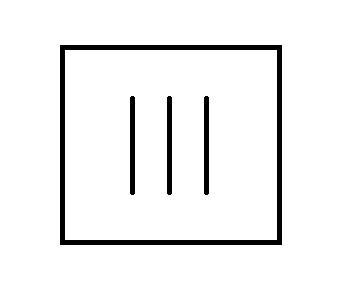
\includegraphics[height=2cm]{chistsquare.jpeg}
\end{figure}

\section{Problemas}

\begin{problem}
    Indiana Jones tiene que cruzar un puente de cuerda que está 
    sobre un barranco de un kilómetro de largo. Está tan oscuro que es 
    imposible cruzar el puente sin una antorcha. Además, el puente es tan 
    débil que no soporta el peso de más de dos personas. 
    El grupo solo tiene una antorcha que ilumina muy poco, por lo que 
    cuando dos personas cruzan, se ven obligadas a cruzar juntas a la 
    velocidad de la persona más lenta. Indiana Jones puede cruzar el 
    puente en 5 minutos, su novia en 10, su amigo en 20 minutos y 
    su padre en 25 minutos. Todos deben estar a salvo antes de que pase 
    una hora para escapar de los chicos malos. ¿Pueden hacerlo?
\end{problem}

\begin{problem}
    Encuentra el número que sigue en la siguiente secuencia:
    \[1, 11, 21, 1211, 111221, \dots\]
\end{problem}

\begin{problem}
    Forma siete triángulos equiláteros con 9 lápices iguales.  
\end{problem}

\begin{problem}
    Tres mujeres llegan a un hotel. El precio anunciado por un día 
    en una sola habitación es de $27$ dólares. Cada una le da $10$ dolares 
    a la portera, pero no tiene cambio así que queda de llevarles más tarde 
    los tres dólares a su cuarto. Una vez se fueron las tres mujeres, 
    la portera se da cuenta de que el precio es en realidad de $25$ dólares 
    la noche. Entonces, deja $25$ dólares en el escritorio, y va a la habitación 
    de las mujeres. Solo le regresa a cada una un dolar, sin decirles el 
    precio verdadero de la habitación. Así que, la portera se embolsó $2$ 
    dólares, mientras que cada hospedada gastó $10-1=9$ dólares, un total de 
    $2 +3  \times 9 = 29$. ¿Qué le pasó al otro dolar?
\end{problem}

\begin{problem}
    Rafa quiere meter una espada de 1.5 metros en un tren pero el conductor 
    no lo dejará llevarla como equipaje de mano. Y, 
    la encargada del equipaje no le permitirá meter ningun objeto 
    cuya dimensión más grande exceda un metro. ¿Qué debe hacer Rafa?
\end{problem}

\begin{problem}

    \rod

    Considera una red finita de pelotas, donde algunas de ellas 
    están unidas por un cable. Podemos colorear cada pelota de azul o 
    rojo , y llamamos a una red "integrada" si cada pelota azul 
    tiene al menos tantos vecinos rojos como azules, y vice versa. 
    Para cualquier red dada, ¿existe una coloración que la integre? 
\end{problem}